% SVN info for this file
\svnidlong
{$HeadURL$}
{$LastChangedDate$}
{$LastChangedRevision$}
{$LastChangedBy$}

\chapter{Convergenza di funzioni}
\labelChapter{convergenzafunzioni}

\begin{introduction}
	‘‘BEEP BOOP QUESTA È UNA CITAZIONE.''
	\begin{flushright}
		\textsc{Marinobot,} dopo aver finito le citazioni stupide.
	\end{flushright}
\end{introduction}
\lettrine[findent=1pt, nindent=0pt]{L}{e} \textbf{[COMPLETARE]} % TO DO: completare l'intro
\section{Convergenza uniforme di funzioni}
Per poter trattare i problemi enunciati nel \refChapterOnly{ellipseintroduction} dobbiamo parlare di convergenza di funzioni. Innanzitutto, ricordiamo le definizioni di distanza, spazio metrico e convergenza.
\begin{define}[Spazio metrico e distanza]
	Uno \textbf{spazio metrico}\index{spazio!metrico} è una coppia $\left(X,\ d\right)$ dove $X$ è un insieme e $\funz{d}{X\times X}{\realset^+}$ è una funzione detta \textbf{distanza}\index{distanza}, cioè tale che $\forall x,\ y,\ z\in X$ essa soddisfi le seguenti proprietà:
	\begin{enumerate}
		\item $\mvf{d}{x}{y}\geq 0,\ \mvf{d}{x}{y}=0\iff x=y$.
		\item $\mvf{d}{x}{y}=\mvf{d}{y}{x}$.
		\item $\mvf{d}{x}{y}\leq\mvf{d}{x}{z}+\mvf{d}{z}{y}$.
	\end{enumerate}
\end{define}
\begin{define}[Convergenza di successioni secondo una distanza]
	Una successione $v_n\in X$ \textbf{converge}\index{convergenza!di una successione} in $X$ a $v\in X$ se
	\begin{equation}
		\forall \epsilon >0,\ \exists N=N\left(\epsilon\right)\colon \forall n\geq N,\ \mvf{d}{v_n}{v}<\epsilon
	\end{equation}
\end{define}
Un \textit{caso particolare} di spazio metrico è lo spazio $X=\mathcal{C}\left(\left[a,b\right];\ \realset\right)$ delle funzioni continue su un intervallo compatto con la \textbf{metrica lagrangiana}\index{metrica!lagrangiana}:
\begin{equation}
	\mvf{d}{f}{g}=\max_{x\in\left[a,b\right]}\abs{f\left(x\right)-g\left(x\right)}
\end{equation}
\begin{observe}
	La distanza è ben definita perché la funzione $\abs{f\left(x\right)-g\left(x\right)}$, essendo definita su $\left[a,b\right]$ compatto, non si considera solo l'estremo superiore ma ammette massimo per il teorema di Weierstrass.
\end{observe}
\begin{define}[Convergenza nella metrica lagrangiana]
	Siano $f_n,\ f\in X$. Si dice che $f_n$ converge a $f$ in $X$ se
	\begin{equation}
		\forall \epsilon >0,\ \exists N=N\left(\epsilon\right)\colon \forall n\geq N,\ \max_{x\in\left[a,b\right]}\abs{f_n\left(x\right)-f\left(x\right)}<\epsilon
		\end{equation}
	\end{define}
	Siccome vale per il massimo allora vale per qualsiasi $x$, quindi la relazione si può riscrivere come
\begin{equation*}
	\forall \epsilon >0,\ \exists N=N\left(\epsilon\right)\colon \forall n\geq N,\ \abs{f_n\left(x\right)-f\left(x\right)}<\epsilon,\ \forall x\in\left[a,b\right]
\end{equation*}
\begin{observe}\label{convergenzalagrangianaeuniforme}
	La condizione, riscritta in questo modo, non solo \textit{non necessita} più dell'esistenza del \textit{massimo}, ma non è neanche necessario che l'intervallo sia \textit{compatto} o che le funzioni $f_n$ siano \textit{continue}: questa è in realtà una relazione \textit{più generale} rispetto alla semplice convergenza nella metrica lagrangiana!\\
	Vedremo che nel caso di funzioni continue sui compatti la convergenza uniforme coincide con quella lagrangiana.
\end{observe}
\begin{define}[Convergenza uniforme]
	Siano $\funz{f_n,\ f}{A\subseteq\realset}{\realset}$ con $A\subseteq R$ qualsiasi. Si dice che $f_n$ \textbf{converge uniformemente}\index{convergenza!uniforme} a $f$\textbf{su} $A$ se
\begin{equation}
	\forall \epsilon >0,\ \exists N=N\left(\epsilon\right)\colon \forall n\geq N,\ \abs{f_n\left(x\right)-f\left(x\right)}<\epsilon,\ \forall x\in A
\end{equation}
\end{define}
\begin{define}[Funzione limite]
	Se $f_n$ converge a $f$ su $A$, $f$ si dice \textbf{funzione limite}\index{funzione!limite}.
\end{define}
\begin{observe}
	Segue immediatamente dalla definizione che se $f_n$ converge uniformemente a $f$ su $A$, allora $\forall B\subseteq A$ si ha che $f_n$ converge uniformemente a $f$ su $B$.
\end{observe}
\begin{attention}
	È estremamente importante dire \textbf{dove} converge $f_n$: infatti, una stessa successione può convergere uniformemente su $A$, ma allo stesso tempo \textit{non convergere} uniformemente in un altro insieme $B$. Vedremo un esempio fondamentale a riguardo successivamente.
\end{attention}
Ora passiamo da questa definizione ad una formulazione equivalente \textit{operativa}.
Se essa vale per qualsiasi $x$ in $A$, allora vale per il $\sup$ e viceversa, quindi è equivalente a dire che
\begin{equation*}
	\forall \epsilon >0,\ \exists N=N\left(\epsilon\right)\colon \forall n\geq N,\ \sup_{x\in A}\abs{f_n\left(x\right)-f\left(x\right)}<\epsilon
\end{equation*}
Siccome il $\sup$ dipende da $n$, possiamo definire una successione
\begin{equation*}
	c_n\coloneqq\sup_{x\in A}\abs{f_n\left(x\right)-f\left(x\right)}\in\realset^+
\end{equation*}
Allora la relazione sopra, per definizione di limite di una successione, è equivalente a $\displaystyle \lim_{n\to+\infty}c_n=0$, cioè
\begin{equation*}
\lim_{n\to+\infty}\left(\sup_{x\in A}\abs{f_n\left(x\right)-f\left(x\right)}\right)=0
\end{equation*}
In conclusione abbiamo mostrato che
\begin{equation}
	f_n\text{ converge uniformemente a }f\text{ in }A\iff\lim_{n\to+\infty}\left(\sup_{x\in A}\abs{f_n\left(x\right)-f\left(x\right)}\right)=0
\end{equation}
\begin{example}\label{valoreassolutoesempioconvergenzaassoluta}
	Proviamo che $f_n\left(x\right)=\sqrt{x^2+\frac{1}{n}}$ converge uniformemente a $f\left(x\right)=\abs{x}$ su $\realset$.\\
	Operativamente, dobbiamo dimostrare che
	\begin{equation*}
		\lim_{n\to+\infty}\left(\sup_{x\in \realset}\abs{f_n\left(x\right)-f\left(x\right)}\right)=0
	\end{equation*}
	\begin{enumerate}
		\item Calcoliamo il $\sup$ con $n$ \textit{fissato}:
		\begin{equation*}
			\sup_{x\in \realset}\abs{f_n\left(x\right)-f\left(x\right)}=\sup_{x\in \realset}\abs{\sqrt{x^2+\frac{1}{n}}-\abs{x}}\stackrel{\ast}{=}\sup_{x\in \realset}\left(\sqrt{x^2+\frac{1}{n}}-\abs{x}\right)
		\end{equation*}
		dove $(\ast)$ si ha perché l'argomento del valore assoluto è sempre positivo.\\
		Per trovare il $\sup$ tracciamo il grafico di $\phi_n\left(x\right)=\abs{\sqrt{x^2+\frac{1}{n}}-\abs{x}}$ e cerchiamo il suo estremo superiore. Per parità della funzione ci basta fare le nostre considerazioni su $\left(0,+\infty\right)$ per poi disegnare il resto del grafico grazie alla simmetria assiale rispetto all'asse $y$; studiando opportunamente la derivata e il limite all'infinito si ottiene il seguente grafico.
\begin{center}
	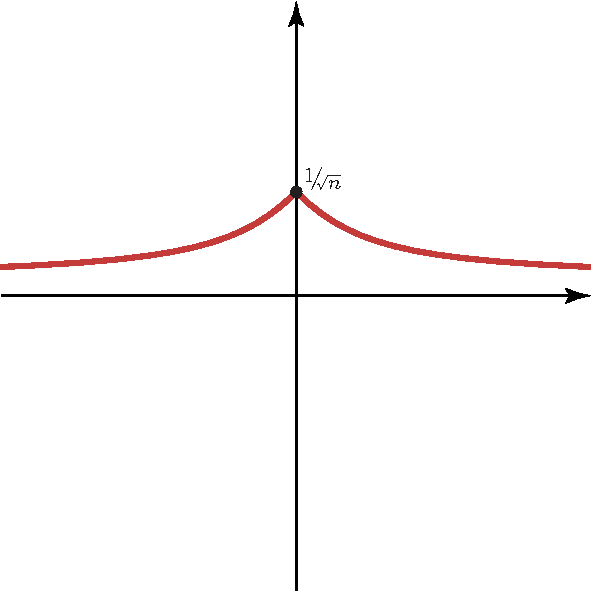
\includegraphics[trim=0cm 4cm 0cm 0cm, clip, scale=0.8]{images/grafico1.pdf}
\end{center}
		Segue chiaramente che
		\begin{equation*}
			\sup_{x\in \realset}\phi_n\left(x\right)=\phi_n\left(0\right)=\frac{1}{\sqrt{n}}\left( =c_n\right)
		\end{equation*}
	\item Calcoliamo il limite per $n\to +\infty$:
	\begin{equation*}
		\lim_{n\to+\infty}\left(\sup_{x\in A}\abs{f_n\left(x\right)-f\left(x\right)}\right)=\lim_{n\to+\infty}\frac{1}{\sqrt{n}}=0
	\end{equation*}
	\end{enumerate}
Abbiamo così verificato la convergenza richiesta.
\end{example}
\begin{examplewt}[Successione geometrica]
	Consideriamo $f_n\left(x\right)=x^n,\ \forall n\geq 0$. Allora:
	\begin{enumerate}
		\item[1.] $x^n$ converge uniformemente a $0$ su \textit{ogni} insieme $\left[-a,a\right],\ \forall a\colon 0<a<1$.
		\item[2.] $x^n$ \textbf{non} converge uniformemente a $0$ su $\left(-1,1\right)$.
	\end{enumerate}
\end{examplewt}
\begin{demonstration}~{}
	\begin{enumerate}
		\item Sia $a\in\left(0,1\right)$ fissato e consideriamo
		\begin{equation*}
			\abs{x^n-0}=\abs{x^n}\implies\sup_{x\in \left[-a,a\right]}\abs{x^n-0}=\sup_{x\in \left[-a,a\right]}\abs{x^n}
		\end{equation*}
		Qual è il grafico di $x^n$?\\
		\begin{minipage}{0.75\textwidth}
			\begin{itemize}
				\item Se $n$ \textbf{pari}, è visivamente simile a quello di $x^2$.
			\end{itemize}
		\end{minipage}\hspace{-7mm}
		\begin{minipage}{0.15\textwidth}
			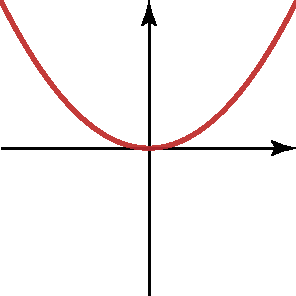
\includegraphics[trim=0cm 0cm 0cm 0cm, clip, scale=0.5]{images/grafico2a.pdf}
		\end{minipage}\\
			\begin{minipage}{0.75\textwidth}
		\begin{itemize}
			\item Se $n$ \textbf{dispari}, è visivamente simile a quello di $x^3$.
		\end{itemize}
	\end{minipage}\hspace{-7mm}
	\begin{minipage}{0.15\textwidth}
		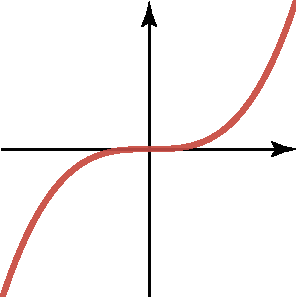
\includegraphics[trim=0cm 0cm 0cm 0cm, clip, scale=0.5]{images/grafico2b.pdf}
	\end{minipage}\\

		Siccome $\abs{x^n},\ \forall n\geq 2$ è una funzione pari, il grafico è visivamente simile a quello di $x^2$.
		Segue immediatamente che
		\begin{equation*}
			\sup_{x\in \left[-a,a\right]}\abs{x^n}=a^n,\ \forall a\colon 0<a<1
		\end{equation*}
		Ora si ha
		\begin{equation*}
			\lim_{n\to+\infty}\left(\sup_{x\in \left[-a,a\right]}\abs{x^n}\right)=\lim_{n\to+\infty}a^n=0
		\end{equation*}
		perché $a\in\left(0,1\right)$ e quindi $a^n$ è una successione geometrica convergente e pertanto il limite a $+\infty$ è sempre necessariamente $0$.
		\item In questo caso anche se non ho il massimo ho l'estremo superiore
		\begin{equation*}
			\sup_{x\in\left(-1,1\right)}\abs{x^n}=1,\ \forall n
		\end{equation*}
		da cui
		\begin{equation*}
			\lim_{n\to+\infty}\left(\sup_{x\in\left(-1,1\right)}\abs{x^n}\right)=1\neq 0
		\end{equation*}
	pertanto \textit{non} c'è convergenza uniforme su $\left(-1,1\right)$.\qedhere
	\end{enumerate}
\end{demonstration}
\subsection{Eserciziamoci! Convergenza uniforme}
\begin{exercise}
	$f_n\left(x\right)=\frac{x^n}{n}$ converge uniformemente a $0$ su $\left[0,1\right]$?
\end{exercise}
\begin{solution}
	Dimostriamo che
	\begin{equation*}
		\lim_{n\to+\infty}\left(\sup_{x\in \left[0,1\right]}\abs{\frac{x^n}{n}-0}\right)=\lim_{n\to+\infty}\left(\sup_{x\in \left[0,1\right]}\frac{x^n}{n}\right)=0
	\end{equation*}
	Poiché
	\begin{equation*}
		\sup_{x\in \left[0,1\right]}\frac{x^n}{n}=\left.\frac{x^n}{n}\right\vert_{x=1}\,=\frac{1}{n}
	\end{equation*}
	allora
	\begin{equation*}
	\lim_{n\to+\infty}\left(\sup_{x\in \left[0,1\right]}\frac{x^n}{n}\right)=\lim_{n\to+\infty}\frac{1}{n}=0
	\end{equation*}
\end{solution}
\subsection{Criterio di Cauchy per la convergenza uniforme}
Come nel caso delle successioni numeriche, esiste un \textbf{criterio di Cauchy} per la convergenza uniforme.
\begin{theoremaqed}[Criterio di Cauchy per la convergenza uniforme]\label{criteriodicauchyperconvergenzauniforme}\index{criterio!di Cauchy!per la convergenza uniforme}
Siano $\funz{f_n}{A\subseteq\realset}{\realset}$. Allora $f_n$ converge uniformemente su $A$ se e solo se
	\begin{equation}
		\forall \epsilon >0,\ \exists N=N\left(\epsilon\right)\colon\forall n,m\geq N,\ \abs{f_n\left(x\right)-f_m\left(x\right)}<\epsilon,\ \forall x\in A\qedhere
	\end{equation}
\end{theoremaqed}
\begin{observe}
Il criterio di Cauchy è un \textit{risultato teorico molto importante}, in quanto permette di mostrare la convergenza uniforme di una successione di funzioni \textit{senza sapere} quale sia il limite come invece è necessario nella definizione di convergenza, in modo analogo a ciò che succede con il criterio di Cauchy per le \textit{successioni numeriche}.
\end{observe}
\subsection{Visualizzazione della convergenza uniforme}
Siamo abituati alle successioni numeriche $v_n$ ed eventualmente a studiare il loro andamento in modo grafico, rappresentando sulle ascisse il numero $n$ e sulle ordinate il valore $v_n$. Nel caso di successioni di funzioni l'argomento è una funzione, quindi per studiarle può essere utile proprio disegnare i grafici degli $f_n$, vedere come cambiano al variare di $n$ e come convergono verso $f$.\\
Come appare \textit{visivamente} la convergenza uniforme? Possiamo riscrivere la condizione della convergenza uniforme
\begin{equation*}
	\forall \epsilon>0,\ \exists N=N\left(\epsilon\right),\ \forall n\geq N,\ \abs{f_n\left(x\right)-f\left(x\right)}<\epsilon,\ \forall x\in A
\end{equation*}
come
\begin{equation}
	f\left(x\right)-\epsilon<f_n\left(x\right)<f\left(x\right)+\epsilon,\ \forall x\in A\text{ definitivamente}
\end{equation}
In altre parole, scelto $\epsilon$, trovo un $N$ nella successione tale che definitivamente $f_n$ deve essere compresa nell'\textbf{intorno tubulare} di $f\left(x\right)$, cioé le $f_n$ devono stare in questo intorno per ogni $n$ sufficientemente grande ($\forall n\geq N$), quindi la striscia cattura globalmente tutte le $f_n$ da un certo $N$ in poi.
\begin{center}\label{visualizzazioneconvergenzauniforme}
	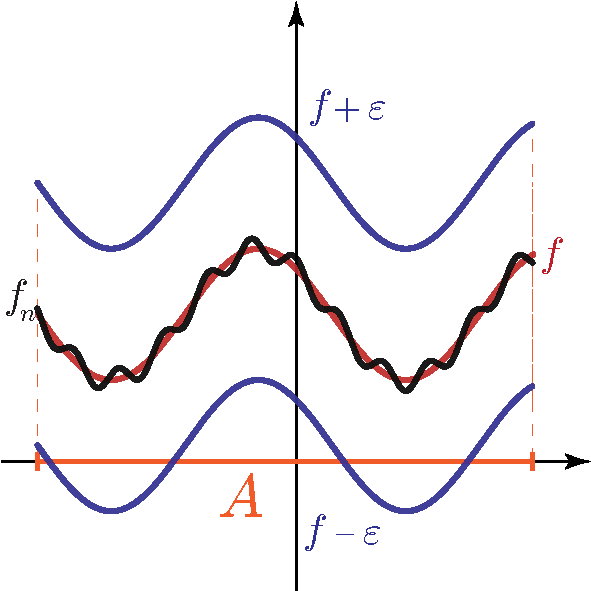
\includegraphics[trim=0cm 0cm 0cm 0cm, clip, scale=0.65]{images/visualizzazioneconvergenzauniforme.pdf}
\end{center}
Visivamente la successione geometrica non converge uniformemente su $(-1,1)$ a $0$ perché non posso restringermi intorno alla funzione limite $f(x)=0$ per qualsiasi $\epsilon$ io scelga, infatti $f_n(1)=1, \forall n$.

\begin{define}[Intorno tubulare]
Un \textbf{intorno tubulare}\index{intorno!tubulare} di larghezza $\epsilon$ di una curva è l'unione di tutti i dischi di raggio $\epsilon$ con centro un punto di una curva.
\end{define}
\subsection{Generalizzazioni della convergenza uniforme}\label{sec:generalizzazioni-della-convergenza-uniforme}
Prima di tutto, ricordiamo le definizioni di norma e spazio normato.
\begin{define}[Spazio normato e norma]
	Uno \textbf{spazio normato}\index{spazio!normato} è una coppia $\left(X,\ \norm{\cdot}\right)$ dove $X$ è un spazio vettoriale su $\kamp$ reale o complesso e $\funz{\lvert\lvert\cdot\rvert\rvert}{X}{\realset^+}$ è una funzione detta \textbf{norma}\index{norma}, cioè tale che $\forall x,\ y\in X,\ \lambda\in\kamp$ essa soddisfi le seguenti proprietà:
	\begin{enumerate}
		\item $\norm{x}\geq 0,\ \norm{x}=0\iff x=0$.
		\item $\norm{\lambda x}=\abs{\lambda}\norm{x}$.
		\item $\norm{x+y}\leq\norm{x}+\norm{y}$.
	\end{enumerate}
\end{define}
	\begin{observe}
	Ogni spazio normato è anche uno spazio metrico se consideriamo la \textbf{metrica indotta dalla norma}\index{metrica!indotta dalla norma}, cioè la funzione data da $\mvf{d}{x}{y}\coloneqq\norm{x-y}$.
\end{observe}
Generalizziamo la definizione di convergenza uniforme considerando $\funz{f_n,\ f}{A}{Y}$, con $A$ \textit{insieme qualsiasi} e $Y$ uno spazio \textit{normato}; se vogliamo che valga anche il criterio di Cauchy è necessario che $Y$ sia \textit{anche} uno spazio \textbf{completo}.
\begin{define}[Successione di Cauchy]
		Una successione $v_n\in X$ è \textbf{di Cauchy}\index{successione!di Cauchy} in $X$ se
	\begin{equation}
		\forall \epsilon >0,\ \exists N=N\left(\epsilon\right)\colon \forall n,m\geq N,\ \mvf{d}{v_n}{v_m}<\epsilon
	\end{equation}
\end{define}
\begin{define}[Spazio completo]
	Uno spazio metrico è detto \textbf{completo}\index{spazio!metrico!completo} se tutte le successioni di Cauchy convergono.
\end{define}
\begin{observe}
	Una successione convergente è \textit{sempre} di Cauchy, ma in generale \textit{non tutte} le successioni di Cauchy convergono. L'implicazione opposta è vera solo se lo spazio è completo.
\end{observe}
Possiamo ora, date queste nuove ipotesi, riformulare la convergenza uniforme.
\begin{define}[Convergenza uniforme, generalizzata]
		Siano $\funz{f_n,\ f}{A}{Y}$ con $A$ insieme qualsiasi e $Y$ spazio normato completo. Si dice che $f_n$ \textbf{converge uniformemente}\index{convergenza!uniforme} a $f$ \textbf{su} $A$ se
	\begin{equation}
		\forall \epsilon >0,\ \exists N=N\left(\epsilon\right)\colon \forall n\geq N,\ \norm{f_n\left(x\right)-f\left(x\right)}<\epsilon,\ \forall x\in A
	\end{equation}
\end{define}
\begin{digression}
	Volendo è possibile generalizzare ulteriormente parlando di convergenza uniforme per funzioni a valori in semplici \textbf{spazi metrici} (completi), sostituendo a $\norm{f_n\left(x\right)-f\left(x\right)}<\epsilon$ la condizione $\mvf{d}{f_n\left(x\right)}{f\left(x\right)}<\epsilon$, infatti se non ci si trova in uno spazio vettoriale potrebbe non essere definita la differenza. Nei nostri studi non affronteremo ciò e ci limiteremo a considerare il caso di spazi normati (completi).
\end{digression}
\section{Convergenza puntuale}
Durante gli studi di \textsc{Calcolo delle probabilità} si è parlato di tre tipi di convergenze di successioni di variabili aleatorie: la \textbf{convergenza in probabilità}, la \textbf{convergenza quasi certa} e la \textbf{convergenza in legge} (o in distribuzione). Consideriamo ora quest'ultima, di cui riportiamo la definizione.
\begin{define}[Convergenza in legge]
	Dato $\left(\Omega,\ \mathcal{M},\ \mathbb{P}\right)$ spazio di probabilità e le variabili aleatorie $\funz{X_n,\ X}{\Omega}{\realset}$ con le corrispettive \textit{funzioni di distribuzione}
	\begin{gather*}
		\funztot{F_n}{\realset}{\realset}{x}{F_n\left(x\right)=\mathbb{P}\left(X_n\leq x\right),\ \forall x\in \realset}\\
		\funztot{F}{\realset}{\realset}{x}{F\left(x\right)=\mathbb{P}\left(X\leq x\right),\ \forall x\in \realset}
	\end{gather*}
allora si dice che $X_n$ converge a $X$ \textbf{in legge}\index{convergenza!in legge} $\left(X_n\stackrel{d}{\to}X\right)$ se
\begin{equation}
	\lim_{n\to+\infty}F_n\left(x\right)=F\left(x\right),\ \forall x\in\realset\ \text{punto di continuità di }F.
\end{equation}
\end{define}
Quello che abbiamo appena scritta non è altro che il caso applicato agli \textit{studi probabilistici} della \textbf{convergenza puntuale} di una successione nel punto $x$.
\begin{define}[Convergenza puntuale]
	Siano $\funz{f_n,\ f}{A}{Y}$ con $A$ insieme qualsiasi e $Y$ spazio normato (completo). $f_n$ converge a $f$ \textbf{puntualmente}\index{convergenza!puntuale} in ogni punto di $A$ se
	\begin{equation}
		\forall x\in A,\ \forall \epsilon>0,\ \exists N=N\left(\epsilon,x\right)\colon\forall n\geq N,\ \norm{f_n\left(x\right)-f\left(x\right)}<\epsilon
	\end{equation}
\end{define}
Confrontiamo qui $\funz{f_n,\ f}{A\subseteq R}{\realset}$:
\begin{enumerate}
	\item \textbf{(CU)} $f_n$ converge a $f$ \textbf{uniformemente} su $A$ se
	\begin{equation*}
		\forall \epsilon>0,\ \exists N=N\left(\epsilon\right)\colon\forall n\geq N,\ \abs{f_n\left(x\right)-f\left(x\right)}<\epsilon,\ \forall x\in A
	\end{equation*}
	\item \textbf{(CP)} $f_n$ converge a $f$ \textbf{puntualmente} in ogni punto di $A$ se
	\begin{equation*}
		\forall x\in A,\ \forall \epsilon>0,\ \exists N=N\left(\epsilon,x\right)\colon\forall n\geq N,\ \abs{f_n\left(x\right)-f\left(x\right)}<\epsilon
	\end{equation*}
\end{enumerate}
Il quantificatore esistenziale $\exists$ implica che ciò che esiste dipende da tutto ciò che lo precede: nella convergenza puntuale $N$ non dipende dal solo $\epsilon$ come così capita nella \textbf{convergenza uniforme}, ma anche da $x$. La convergenza uniforme è più restrittiva rispetto alla puntuale perché la soglia $N$ è indipendente da $x$, quindi basta trovare un solo $N$ che va bene per tutte le $x\in A$ (ed è questo il motivo per cui $\forall x\in A$ appare al fondo della formula), al contrario della convergenza puntuale in cui la soglia $N$ dipende dalla $x$ che consideriamo.

\begin{observe}
	Questa differenza è concettualmente analoga a quella che c'è fra continuità uniforme e continuità.
\end{observe}
\begin{observe}
	Possiamo considerare $\forall \epsilon >0$ due punti $x'$ e $x''$ su cui valutare la \textbf{soglia} $N$ di un successione di funzioni: in questo caso abbiamo per il primo punto $N\left(\epsilon,\ x'\right)$ e per il secondo $N\left(\epsilon,\ x''\right)$. Vediamo subito che $\max\left(N\left(\epsilon,\ x'\right),N\left(\epsilon,\ x''\right)\right)$ è una soglia lecita sia per $x'$ sia $x''$.\\
	Finché si ha un numero finito di punti si può considerare il massimo, ma in generale se voglio passare dalla convergenza puntuale alla convergenza uniforme avendo un numero infinito di punti devo considerare
	\begin{equation*}
		\sup_{x\in A}N\left(\epsilon, x\right)
	\end{equation*}
\begin{itemize}
	\item Se $\displaystyle\sup_{x\in A}N\left(\epsilon\right)$ è finito, allora $\displaystyle\sup_{x\in A}N\left(\epsilon\right)=\max_{x\in A}N\left(\epsilon\right)=N\left(\epsilon\right)$ e c'è convergenza uniforme.
	\item Se $\displaystyle\sup_{x\in A}N\left(\epsilon\right)=+\infty$ allora \textit{non} c'è convergenza uniforme.
\end{itemize}
\end{observe}
Dalle definizioni segue immediatamente che\label{convuniformeimplicapuntuale}
	\begin{multline}
	f_n\text{ converge uniformemente a }f\text{ su }A\implies\\
	\implies f_n\text{ converge puntualmente a }f\text{ in ogni punto di }A
\end{multline}
ma in generale vale che la convergenza puntuale \textbf{non} implica la convergenza uniforme perché fissata la tolleranza $\epsilon$ la soglia $N$ potrebbe cambiare al variare di $x\in A$.
\begin{examplewt}[Successione geometrica e convergenza puntuale]
	Consideriamo la successione geometrica $f_n\left(x\right)=x^n,\ \forall n\geq 0$.\\
	Dagli studi fatti nel corso di \textsc{Analisi 1} si ha $\forall x\in\realset$ fissato 
	\begin{equation*}
		\lim_{n\to+\infty}x^n=
		\begin{cases}
			\begin{array}{ll}
				+\infty&\text{se }x>1\\
				1&\text{se }x=1\\
				0&\text{se }-1<x<1\\
				\text{non esiste}&\text{se }x\leq 1
			\end{array}
		\end{cases}
	\end{equation*}
Allora $x^n$ converge puntualmente a
\begin{equation*}
	f\left(x\right)=
	\begin{cases}
	1&\text{se }x=1\\
	0&\text{se }-1<x<1	
	\end{cases}
\end{equation*}
in ogni punto di $\left(-1,1\right]$ e la funzione limite è discontinua.
\begin{center}
	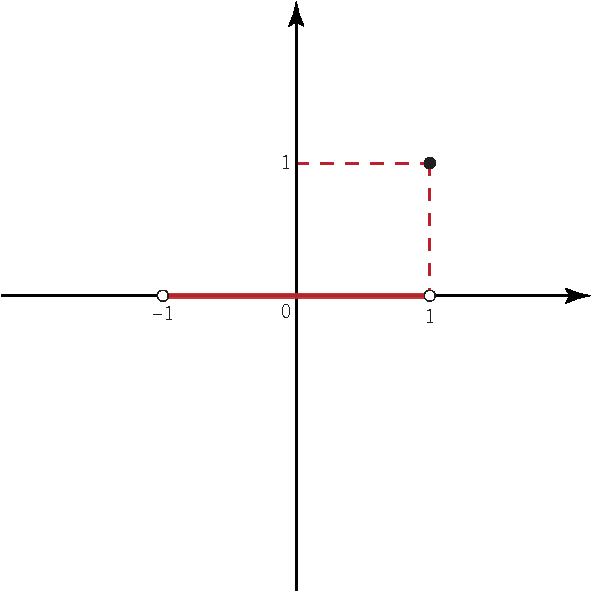
\includegraphics[trim=0cm 4cm 0cm 0cm, clip, scale=0.65]{images/grafico4.pdf}
\end{center}
\end{examplewt}
Abbiamo provato precedentemente che $f_n\left(x\right)=x^n$ converge uniformemente a $f\equiv 0$ in ogni intervallo $\left[-a,a\right]\subsetneqq\left(-1,1\right),\ \forall a\in\left(0,1\right)$, ma \textit{non} converge uniformemente a $f\equiv0$ in $\left(-1,1\right)$. Questo mostra che su $\left(-1,1\right)$ c'è convergenza puntuale ma non uniforme.
\begin{observe}
	Questo esempio mostra inoltre che la convergenza puntuale \textit{non} è sufficiente in generale per trasferire la continuità alla funzione limite.
\end{observe}
\section{Proprietà di regolarità nel caso di convergenza uniforme e puntuale}
Adesso studiamo il diverso comportamento delle due tipologie di convergenza viste rispetto alle proprietà di regolarità: se le funzioni $f_n$ della successione sono limitate/continue/integrabili/differenziabili, la funzione limite $f$ è limitata/continua/integrabile/differenziabile?
\subsection{Limitatezza}
\begin{theorema}[Teorema di limitatezza per successioni]
Siano $\funz{f_n,f}{\left[a,b\right]}{\realset},\ n\geq 1$ tali che
\begin{enumerate}
	\item $f_n$ limitata su $\left[a,b\right],\ \forall n\geq 1$.
	\item $f_n$ converge uniformemente a $f$ su $\left[a,b\right]$.
\end{enumerate}
Allora $f$ è limitata su $\left[a,b\right]$.
\end{theorema}
\begin{demonstration}
	Dobbiamo provare e $f$ è limitate, ovvero che
	\begin{equation*}
		\exists M>0\colon \abs{f(x)}\leq n,\ \forall x\in A
	\end{equation*}
Per l'ipotesi $2)$ sappiamo che
\begin{equation*}
	\forall \epsilon>0,\ \exists N=N\left(\epsilon\right)\colon\forall n\geq N,\ \abs{f_n\left(x\right)-f\left(x\right)}<\epsilon,\ \forall x\in A
\end{equation*}
Posto ad esempio\footnote{La scelta di $\epsilon$ è arbitraria.} $\epsilon = 2$, consideriamo la soglia $N_2=N\left(2\right)$ e $n=N_2$. Allora la relazione precedente risulta
\begin{equation*}
	\abs{f_{N_2}\left(x\right)-f\left(x\right)}<2,\ \forall x\in A
\end{equation*}
Consideriamo $f_{N_2}\left(x\right)$: per l'ipotesi $1)$ è limitata, cioè
\begin{equation*}
	\exists M_2>0\colon \abs{f_{N_2}(x)}\leq M_2,\ \forall x\in A
\end{equation*}
Per ogni $x\in A$ si ha quindi
\begin{equation*}
	\abs{f\left(x\right)}=\abs{f\left(x\right)+f_{N_2}(x)-f_{N_2}(x)}\leq\abs{f\left(x\right)-f_{N_2}(x)}+\abs{f_{N_2}(x)}\leq 2+M_2=M,\ \forall x\in A\qedhere
\end{equation*}
\end{demonstration}
\begin{digression}
	Il risultato si generalizza ponendo $\funz{f_n,f}{X}{Y}$, dove $X$ è un qualunque insieme e $Y$ è uno spazio normato.
\end{digression}
La convergenza puntuale non è sufficiente per trasferire la limitatezza alla funzione limite: infatti, possiamo costruire un controesempio di una successione $f_n$ limitata che converge puntualmente ad una funzione non limitata.
\begin{example}
	Sia $\funz{f_n}{\left(0,1\right]}{\realset},\ n\geq1$, definita da
	\begin{equation*}
		f_n\left(x\right)=\begin{cases}
			\begin{array}{ll}
				n&\text{se }0<x<\frac{1}{n}\\
				\frac{1}{x}&\text{se }x\geq\frac{1}{n}\\
			\end{array}
		\end{cases}
	\end{equation*}
$\forall x\in \left(0,1\right]$.\\
Un grafico qualitativo di $f_n$ è rappresentato in figura.
\begin{center}
	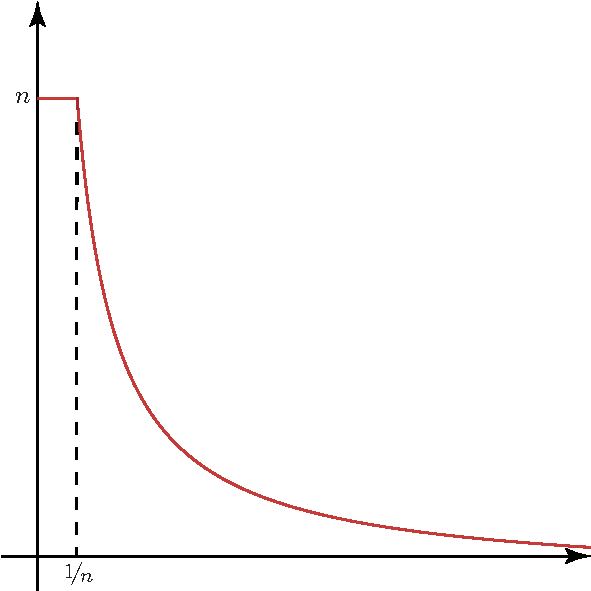
\includegraphics[trim=0cm 0cm 0cm 0cm, clip, scale=0.65]{images/grafico5.pdf}
\end{center}
Per ogni $n\geq1$ la funzione $f_n$ è limitata su $\left(0,1\right]$. Inoltre, $\forall x\in \left(0,1\right]$ si ha
	
	\begin{equation*}
		\lim_{n\to+\infty}f_n\left(x\right)=\frac{1}{x}
	\end{equation*}
	Infatti, fissato $x\in \left(0,1\right]$, indicando con le parentesi quadre la \textit{parte intera} e posto 
	\begin{equation*}
	n_x=\left[\frac{1}{x}\right]+1
	\end{equation*}
	allora se $n\geq n_x$ si ha $x>1/n$ e dunque
	\begin{equation*}
	f_n\left(x\right)=\frac{1}{x}
	\end{equation*}
	Si ha dunque
	\begin{equation*}
		\lim_{n\to+\infty}f_n\left(x\right)=\lim_{n\to+\infty}\frac{1}{x}=\frac{1}{x}
	\end{equation*}
	La successione di funzioni \textit{limitate} $f_n$ converge quindi puntualmente $\forall x\in \left(0,1\right]$ alla funzione $\frac{1}{x}$ che \textbf{non} è limitata su $\left(0,1\right]$.
\end{example}
\subsection{Continuità}
\begin{theorema}[Teorema di continuità per successioni]
	Siano $\funz{f_n,f}{\left[a,b\right]}{\realset},\ n\geq 1$ tali che
	\begin{enumerate}
		\item $f_n$ continua su $\left[a,b\right],\ \forall n\geq 1$.
		\item $f_n$ converge uniformemente a $f$ su $\left[a,b\right]$.
	\end{enumerate}
	Allora $f$ è continua su $\left[a,b\right]$.
\end{theorema}
\begin{demonstration}
	Sia $x_0\in\left[a,b\right]$ fissato. Dobbiamo dimostrare che
	\begin{equation*}
		\forall \epsilon>0,\ \exists \delta>0 \colon \abs{x-x_0}<\delta\implies \abs{f\left(x\right)-f\left(x_0\right)}<\epsilon
	\end{equation*}
	Per l'ipotesi $2)$ sappiamo che $f_n$ converge uniformemente; allora, fissato $\epsilon>0$, $\exists N=N\left(\epsilon\right)\in\naturalset$ tale che
	\begin{equation*}
		\abs{f_N\left(x\right)-f\left(x\right)}<\frac{\epsilon}{3},\ \forall x\in\left[a,b\right]
	\end{equation*}
Questa relazione chiaramente vale anche per $x_0$:
	\begin{equation*}
	\abs{f_N\left(x_0\right)-f\left(x_0\right)}<\frac{\epsilon}{3}
\end{equation*}
Per l'ipotesi $1)$ ogni $f_n$ è continua in $x_0$, in particolare $f_N$ la è. Per definizione di continuità, considerato sempre lo stesso $\epsilon>0$ di prima $\exists\delta >0$ tale che se $\abs{x-x_0}<\delta$ si ha
	\begin{equation*}
	\abs{f_N\left(x\right)-f_N\left(x_0\right)}<\frac{\epsilon}{3}
\end{equation*}
Quindi, se $\abs{x-x_0}<\delta$ abbiamo
\begin{equation*}
	\abs{f\left(x\right)-f\left(x_0\right)}\leq\abs{f\left(x\right)-f_N\left(x\right)}+\abs{f_N\left(x\right)-f_N\left(x_0\right)}+\abs{f_N\left(x_0\right)-f\left(x_0\right)}\leq\frac{\epsilon}{3}+\frac{\epsilon}{3}+\frac{\epsilon}{3}=\epsilon\qedhere
\end{equation*}
\end{demonstration}
\begin{digression}
	Il risultato si generalizza ponendo $\funz{f_n,f}{X}{Y}$, dove $X$ è un qualunque insieme e $Y$ è uno spazio normato.
\end{digression}
La convergenza puntuale non è sufficiente per trasferire la continuità alla funzione limite: infatti, possiamo costruire un controesempio di una successione $f_n$ continua che converge puntualmente ad una funzione non continua.
\begin{example}
Consideriamo la successione geometrica $f_n(x)=x^n,\ n\geq1$, sull'intervallo $[0,1]$.\\
Sappiamo che essa converge puntualmente in ogni punto di $[0,1]$ alla funzione limite 
\begin{equation*}
	f\left(x\right)=
	\begin{cases}
		\begin{array}{ll}
			0&\text{se }0\leq x < 1\\
			1&\text{se }x=1
		\end{array}
	\end{cases}
\end{equation*}
La successione di funzioni \textit{continue} $f_n$ converge quindi puntualmente per ogni $x\in[0,1]$ alla funzione $f$ che \textbf{non} è continua su $[0,1]$.
\end{example}
\subsection{Integrabilità e passaggio al limite sotto segno di integrale}
D'ora in avanti indicheremo con $\mathcal{R}\left(\left[a,b\right]\right)$ l'insieme delle funzioni integrabili secondo Riemann su $[a,b]$.
\begin{theoremaqed}[Teorema di integrabilità per successioni, passaggio al limite sotto segno di integrale]\label{passaggioallimitecontinuitàuniforme}
	Siano $\funz{f_n,f}{\left[a,b\right]}{\realset},\ n\geq 1$ tali che
	\begin{enumerate}
		\item $f_n\in\mathcal{R}\left(\left[a,b\right]\right),\ \forall n\geq 1$.
		\item $f_n$ converge uniformemente a $f$ su $\left[a,b\right]$.
	\end{enumerate}
	Allora
	\begin{enumerate}
		\item $f\in\mathcal{R}\left(\left[a,b\right]\right)$.
		\item Vale il \textbf{passaggio al limite sotto segno di integrale}\index{passaggio al limite sotto segno di integrale}:
		\begin{equation}
			\lim_{n\to+\infty}\int_{a}^{b}f_n\left(x\right)dx=\int_{a}^{b}\lim_{n\to+\infty}f_n\left(x\right)dx=\int_{a}^{b}f\left(x\right)dx\qedhere
		\end{equation}
	\end{enumerate}
\end{theoremaqed}
\begin{observe}
	Nel caso di un intervallo \textit{illimitato} la convergenza uniforme 
	\begin{itemize}
		\item \textit{non} è condizione sufficiente per il passaggio al limite sotto il segno di integrale, e non è necessaria neanche nel caso limitato
		\item \textit{non} è condizione sufficiente per trasferire alla funzione limite l'integrabilità
	\end{itemize}
	Inoltre la convergenza puntuale \textit{non} è condizione sufficiente per il passaggio al limite sotto il segno di integrale, nemmeno nel caso di un intervallo limitato.\\
	Di seguito vedremo dei controesempi.
\end{observe}
Vedremo la dimostrazione di una versione più generica del teorema quando parleremo degli integrali di Lebesgue.
\begin{examples}
	Per quanto questo teorema ha una notevole importanza, ha un campo d'azione particolarmente limitato. Infatti, anche cambiando leggermente le ipotesi non è più possibile affermare la tesi. Vediamo alcuni di questi controesempi.
	\begin{enumerate}
		\item La convergenza \textbf{uniforme} \textit{non} è \textbf{sufficiente} per trasferire alla funzione limite l'integrabilità su un intervallo \textit{illimitato}.
		\item La convergenza \textbf{uniforme} \textit{non} è condizione \textbf{necessaria} per il passaggio al limite sotto segno di integrale.
		\item La convergenza \textbf{uniforme} \textit{non} è condizione \textbf{sufficiente} per il passaggio al limite sotto il segno di integrale nel caso in un intervallo \textit{illimitato}.
		\item La convergenza \textbf{puntuale} \textit{non} è condizione \textbf{sufficiente} per il passaggio al limite sotto il segno di integrale, \textit{nemmeno} nel caso di un intervallo \textit{limitato}.
	\end{enumerate}
\textbf{\textsc{Dimostrazione.}}
\begin{enumerate}[label=\Roman*]
	\item 	Consideriamo la successione di funzioni $\funz{f_n}{\left[1,+\infty\right)}{\realset}$ definite da
	\begin{equation*}
		f_n(x)=\frac{n}{nx+x^2},\ \forall x\geq1, n\geq1 
	\end{equation*}
	Per ogni $x\geq 1$ osserviamo che $f_n(x)\sim \frac{n}{nx}$ per $n\to+\infty$, quindi si ha
	\begin{equation*}
		\lim_{n\to+\infty}f_n\left(x\right)=\lim_{n\to+\infty}\frac{n}{nx}=\frac{1}{x}
	\end{equation*}
	Si ha quindi convergenza puntuale in ogni punto di $\left[1,+\infty\right)$ alla funzione $f(x)=\frac{1}{x}$. Inoltre, la convergenza è uniforme su $\left[1,+\infty\right)$: vale infatti
	\begin{equation*}
		\abs{f_n(x)-f(x)}=\abs{\frac{n}{nx+x^2}-\frac{1}{x}}=\frac{1}{n+x}
	\end{equation*}
	per ogni $x\geq1$, $n\geq1$. Per \textit{monotonia}, si ha quindi
	\begin{equation*}
		\sup_{x\geq 1}\abs{f_n(x)-f(x)}=\sup_{x\geq1}\frac{1}{n+x}=\frac{1}{n+1},\ \forall n\geq1
	\end{equation*}
	Deduciamo che
	\begin{equation*}
		\lim_{n\to+\infty}\left(\sup_{x\geq1}\abs{f_n(x)-f(x)}\right)=\lim_{n\to+\infty}\frac{1}{n+1}=0
	\end{equation*}		
	da cui segue la convergenza uniforme su $\left[1,+\infty\right)$.
	Osserviamo ora che per ogni $n\geq1$ si ha
	\begin{equation*}
		f_n(x)\sim \frac{n}{x^2},\ x\to+\infty
	\end{equation*}
	e dunque $f_n$ è integrabile in senso improprio su $[1,+\infty)$, per ogni $n\geq1$; la funzione limite $f(x)=\frac{1}{x}$ \textit{non} è invece integrabile in senso improprio su $[1,+\infty)$.\\
	La successione di funzioni $f_n$ \textit{integrabili} su $[1,+\infty)$ converge quindi uniformemente su $[1,+\infty)$ alla funzione $f$ che \textbf{non} è integrabile su $[1,+\infty)$.
	\item 	Consideriamo la successione di funzioni $f_n\left(x\right)=x^n$ definite su $\left[0,1\right]$. Osserviamo che
	\begin{equation*}
		\lim_{n\to+\infty}\int_{0}^{1}x^ndx=\lim_{n\to+\infty}\left[\frac{1}{n+1}x^{n+1}\right]_{0}^{1}=\lim_{n\to+\infty}\frac{1}{n+1}=0
	\end{equation*}
	Invece, sappiamo che $x^n$ converge puntualmente in ogni punto di $[0,1]$ alla funzione limite 
	\begin{equation*}
		f\left(x\right)=
		\begin{cases}
			\begin{array}{ll}
				0&\text{se }0\leq x < 1\\
				1&\text{se }x=1
			\end{array}
		\end{cases}
	\end{equation*}
	dunque su $[0,1]$ $\displaystyle f\left(x\right)=\lim_{n\to\infty}f_n\left(x\right)$ è una funzione \textit{identicamente nulla} tranne un \textit{numero finito} di punti (in questo caso, uno soltanto). Allora
	\begin{equation*}
		\int_{0}^{1}\lim_{n\to+\infty}x^ndx=\int_{0}^{1}0dx=0
	\end{equation*}
	$x^n$ non converge uniformemente su $\left[0,1\right]$, ma il passaggio al limite sotto segno di integrale si verifica comunque.
	\item Sia $\funz{f_n}{\left[0,+\infty\right)}{\realset}$, $n\geq1$, definita da
	\begin{equation*}
		f_n\left(x\right)=\begin{cases}
			\begin{array}{ll}
				\frac{1}{n}&\text{se }n\leq x\leq2n\\
				0 &\text{se }x<n\vee x>2n
			\end{array}
		\end{cases}
	\end{equation*}
	Osserviamo che
	\begin{align*}
		\lim_{n\to+\infty}\int_{0}^{+\infty}f_n\left(x\right)dx=&\lim_{n\to+\infty}\left[\int_{0}^{n}0dx+\int_{n}^{2n}\frac{1}{n}dx+\int_{2n}^{+\infty}0dx\right]=\lim_{n\to+\infty}\int_{n}^{2n}\frac{1}{n}dx=\\
		=&\lim_{n\to+\infty}\left[\frac{x}{n}\right]_{n}^{2n}=\lim_{n\to+\infty}\frac{2n-n}{n}=\lim_{n\to+\infty}1=1
	\end{align*}
	Invece, si vede immediatamente che
	\begin{equation*}
		\int_{0}^{+\infty}\lim_{n\to+\infty}f_n\left(x\right)dx=\int_{0}^{+\infty}0dx=0
	\end{equation*}
	Vediamo che $f_n$ converge uniformemente su $\left[0,+\infty\right)$ a $0$:
	\begin{gather*}
		\sup_{x\in\left[0,+\infty\right)}\abs{f_n\left(x\right)-f\left(x\right)}=\frac{1}{n}\\
		\lim_{n\to+\infty}\left(\sup_{x\in\left[0,+\infty\right)}\right)=\lim_{n\to+\infty}\frac{1}{n}=0
	\end{gather*}
	Anche aggiungendo al teorema l'ipotesi che $f\left(x\right)$ sia Riemann-integrabile (in questo caso ciò è verificato), il passaggio al limite sotto segno di integrale \textit{non} si verifica \textit{necessariamente} se l'intervallo è illimitato.
	\item 	Consideriamo la successione di funzioni $f_n\left(x\right)=nx\left(1-x^2\right)^n$ definite su $\left[0,1\right]$. Osserviamo che
	\begin{align*}
		\lim_{n\to+\infty}\int_{0}^{1}nx\left(1-x^2\right)^ndx=&-\frac{1}{2}\lim_{n\to+\infty}\int_{0}^{1}n\left(-2x\right)\left(1-x^2\right)^n=\\
		=&-\frac{1}{2}\lim_{n\to+\infty}n\left[\frac{1}{n+1}\left(1-x^2\right)^{n+1}\right]_{0}^{1}=\frac{1}{2}\lim_{n\to+\infty}\frac{n}{n+1}=\frac{1}{2}
	\end{align*}
	Invece, osserviamo che, se abbiamo fissato $x$ rispetto alla $n$, allora $nx\left(1-x^2\right)^n=x\frac{\left(1-x^2\right)^n}{\frac{1}{n}}$ si può vedere come il rapporto di un esponenziale di ragione (in modulo) minore di 1 con il reciproco di un termine lineare, dunque per $n\to+\infty$ l'esponenziale tende a $0$ molto più velocemente di $\frac{1}{n}$: segue che
	\begin{equation*}
		\int_{0}^{1}\lim_{n\to+\infty}nx\left(1-x^2\right)^ndx=\int_{0}^{1}0dx=0
	\end{equation*}
	Per lo stesso ragionamento si vede che $f_n\left(x\right)$ converge puntualmente a $0$ per ogni punto di $\left[0,1\right]$, ma \textit{non} si verifica il passaggio al limite sotto segno di integrale.\qed
\end{enumerate}
\end{examples}
\subsection{Derivabilità}
Date $\funz{f_n,f}{A\subseteq\realset}{\realset}$ con $f$ la funzione limite di $f_n$ su $A$, possiamo porci due domande:
\begin{enumerate}
	\item $f_n$ derivabile su $A\implies f$ derivabile su $A$?
	\item Vale lo scambio tra derivata e limite?
	\begin{equation*}
		\lim_{n\to+\infty}f'_n\left(x\right)=D\left(\lim_{n\to+\infty}f\left(x\right)\right)
	\end{equation*}
	O, in altre parole, il diagramma seguente è commutativo?
	% https://q.uiver.app/?q=WzAsNCxbMCwwLCJmX24iXSxbMSwwLCJmJ19uIl0sWzAsMSwiXFxsaW1fe25cXHRvK1xcaW5mdHl9Zl9uIl0sWzEsMSwiXFxsaW1fe25cXHRvK1xcaW5mdHl9ZidfbiJdLFswLDEsIkQiXSxbMCwyLCJcXGxpbSIsMl0sWzEsM10sWzIsM11d
\[\begin{tikzcd}
	{f_n} & {f'_n} \\
	{\textcolor{blueill}{\displaystyle\lim_{n\to+\infty}f_n}} & {\displaystyle\lim_{n\to+\infty}f'_n}
	\arrow["D", from=1-1, to=1-2]
	\arrow["\lim"', color={rgb,255:red,46;green,49;blue,146}, from=1-1, to=2-1]
	\arrow["\lim", from=1-2, to=2-2]
	\arrow["D"', color={rgb,255:red,46;green,49;blue,146}, from=2-1, to=2-2]
\end{tikzcd}\]
\end{enumerate}
La risposta ad entrambe domande, a differenza di quanto ci si potrebbe aspettare dati i risultati su limitatezza, continuità e integrabilità, è \textbf{NO}, anche nel caso di \textit{convergenza uniforme}.
\begin{examplewt}[La convergenza uniforme \textit{non} è condizione sufficiente per trasferire alla funzione limite la derivabilità]
Consideriamo la successione $f_n(x)=\sqrt{x^2+\frac{1}{n}},\ \forall x\in \realset,\ \forall n\geq1$.
	\begin{itemize}
		\item $f_n$ è derivabile.
		\item $f_n$ abbiamo visto\footnote{Si veda pag. \pageref{valoreassolutoesempioconvergenzaassoluta}.} converge uniformemente su $\realset$ a $f\left(x\right)=\abs{x}$ che \textit{non} è derivabile in $x=0$.
	\end{itemize}
\end{examplewt}
\begin{examplewt}[La convergenza uniforme \textit{non} è condizione sufficiente per poter scambiare limite e derivata, anche se si aggiunge l'ipotesi che la funzione limite sia derivabile]
	Consideriamo la successione $f_n(x)=\frac{\sin\left(nx\right)}{\sqrt{n}},\ \forall x\in \realset,\ \forall n\geq1$.
	\begin{itemize}
		\item $f_n$ è derivabile su $\realset$, $\forall n\geq 1$, e vale
		\begin{equation*}
			f'\left(x\right)=\sqrt{n}\cos\left(nx\right),\ \forall x\in \realset,\ \forall n\geq1
		\end{equation*}
		\item
		\begin{itemize}
			\item $f_n$ converge \textbf{puntualmente} a $f\left(x\right)=0,\ \forall x\in\realset$:
			\begin{equation*}
				\lim_{n\to+\infty}f_n\left(x\right)=\lim_{n\to+\infty}\underbrace{\frac{1}{\sqrt{n}}}_{\to 0}\underbrace{\sin\left(nx\right)}_{\text{limitato}}=0,\ \forall x\in\realset
			\end{equation*}
			\item $f_n$ converge \textbf{uniformemente} a $f\left(x\right)=0,\ \forall x\in\realset$:
			\begin{equation*}
				\lim_{n\to+\infty}\left(\sup_{x\in\realset}\abs{f_n\left(x\right)-f\left(x\right)}\right)=\lim_{n\to+\infty}\left(\sup_{x\in\realset}\abs{\frac{\sin\left(nx\right)}{\sqrt{n}}}\right)=\lim_{n\to+\infty}\frac{1}{\sqrt{n}}=0
			\end{equation*}
		\end{itemize}
		Osserviamo che in entrambi i casi $f\left(x\right)=0$ su $\realset$: questa funzione è chiaramente derivabile e vale
		\begin{equation*}
			D\left(\lim_{n\to+\infty}f_n\left(x\right)\right)=D\left(0\right)=0,\ \forall x\in\realset
		\end{equation*}
	D'altro canto, si ha
	\begin{equation*}
			\lim_{n\to+\infty}D\left(f_n\left(x\right)\right)=\lim_{n\to+\infty}f'_n\left(x\right)=\lim_{n\to+\infty}\sqrt{n}\cos\left(nx\right)
	\end{equation*}
		Ad esempio, per $x=0$ troveremmo
		\begin{equation*}
				\lim_{n\to+\infty}D\left(f_n\left(x\right)\right)=\lim_{n\to+\infty}\sqrt{n}=+\infty
		\end{equation*}
	Quindi non si può per $x=0$ scambiare limite e derivata-
	\end{itemize}
\end{examplewt}
Esiste comunque un legame tra \textit{successioni di funzioni}, \textit{derivabilità} e convergenza uniforme; scopriamo che non è più la successione $f_n$ a dover convergere uniformemente, bensì sono le derivate $f'$ della successioni a doverlo fare.
\begin{theorema}[Teorema di derivabilità per successioni]
	Siano dati $\funz{f_n}{\left(a,b\right)}{\realset}$ tali che
	\begin{enumerate}
		\item $f_n$ derivabili su $\left(a,b\right)$.
		\item $\exists c\in\left(a,b\right)\colon f_n\left(c\right)$ converge puntualmente.
		\item $f'_n$ converge uniformemente a $g$ su $\left(a,b\right)$.
	\end{enumerate}
Allora
\begin{enumerate}
	\item $\exists\funz{f}{\left(a,b\right)}{\realset}$ tale che $f_n$ converge uniformemente a $f$ su $\left(a,b\right)$.
	\item $f$ è derivabile.
	\item $f'\left(x\right)=g\left(x\right),\ \forall x\in \left(a,b\right)$, ossia
	\begin{equation}
		D\left(\lim_{n\to+\infty}f_n\left(x\right)\right)=\lim_{n\to+\infty}f'_n\left(x\right),\ \forall x\in\left(a,b\right)
	\end{equation}
\end{enumerate}
\end{theorema}
Per dimostrare il teorema, faremo uso di tre strumenti: il \textit{criterio di Cauchy per la convergenza uniforme} \footnote{Si veda il teorema \ref{criteriodicauchyperconvergenzauniforme}, pag. \pageref{criteriodicauchyperconvergenzauniforme}.}, il \textit{teorema di scambio di limiti} e una conseguenza \textit{teorema di Lagrange}. Enunciamo questi ultimi due.
\begin{theoremaqed}[Teorema di scambio di limiti]
	Dati $\funz{g_n,g}{I\subseteq \realset}{\realset}$ e $c$ punto di accumulazione di $I$, se
	\begin{enumerate}
		\item $g_n$ converge \textit{uniformemente} a $g$ su $I$
		\item Per ogni $n \geq 1$ esiste $L_n\in\realset$ tale che
		\begin{equation*}
			\lim_{x\to c}g_n\left(x\right)=L_n
		\end{equation*}
	\end{enumerate}
	Allora:
	\begin{enumerate}
		\item Esistono finiti
		\begin{equation}
				\lim_{x\to c}g\left(x\right),\qquad\lim_{n\to+\infty}L_n
		\end{equation}
		\item Vale la relazione
		\begin{equation}
			\lim_{x\to c}g\left(x\right)=\lim_{n\to+\infty}L_n
		\end{equation}
		ossia
	\begin{equation}
		\lim_{x\to c}\lim_{n\to+\infty}g_n\left(x\right)=\lim_{n\to+\infty}\lim_{x\to c}g_n\left(x\right)\qedhere
	\end{equation}
	\end{enumerate}	
\end{theoremaqed}
\begin{corollaryqed}[Conseguenza al teorema di Lagrange]
Sia $\funz{h}{\left(\alpha,\beta\right)\subseteq\realset}{\realset}$ derivabile in $\left(\alpha,\beta\right)$. Allora:
\begin{equation}
	\forall u,v\in\left(\alpha,\beta\right),\  \abs{h\left(u\right)-h\left(v\right)}\leq\left(\sup_{x\in\left(\alpha,\beta\right)}\abs{h'\left(x\right)}\right)\abs{u-v}\qedhere
\end{equation}
\end{corollaryqed}
\begin{demonstration} \textsc{(del Teorema di derivabilità per successioni.)}
\begin{enumerate}
	\item Dimostriamo la \textit{convergenza uniforme} di $f_n$ su $\left(a, b\right)$. Per il Criterio di Cauchy per la convergenza uniforme è sufficiente
	dimostrare che
	\begin{equation*}
		\forall \epsilon >0,\ \exists N=N\left(\epsilon\right)\colon\forall n,m\geq N,\ \sup_{x\in \left(a,b\right)}\abs{f_n\left(x\right)-f_m\left(x\right)}<\epsilon
	\end{equation*}
Sia $\epsilon>0$. Per ogni $x\in\left(a,b\right)$, preso $c$ come da ipotesi $2)$:
\begin{equation*}
	\abs{f_n\left(x\right)-f_m\left(x\right)}\leq \abs{f_n\left(x\right)-f_m\left(x\right)-\left(f_n\left(c\right)-f_m\left(c\right)\right)}+\abs{f_n\left(c\right)-f_m\left(c\right)}
\end{equation*}
Studiamo il \textit{primo addendo}. Per il \textit{corollario al teorema di Lagrange} si ha
\begin{equation*}
	\abs{f_n\left(x\right)-f_m\left(x\right)-\left(f_n\left(c\right)-f_m\left(c\right)\right)}\leq\left(\sup_{t\in\left(a,b\right)}\abs{x-c}\right)
\end{equation*}
Inoltre, poiché per ipotesi $3)$ $f'_n$ converge uniformemente su $\left(a,b\right)$, si ha per il criterio di Cauchy che
\begin{equation*}
	\forall \epsilon >0,\ \exists N_1=N_1\left(\epsilon\right)\colon\forall n,m\geq N_1,\ \sup_{x\in \left(a,b\right)}\abs{f'_n\left(x\right)-f'_m\left(x\right)}<\frac{\epsilon}{2\left(b-a\right)}
\end{equation*}
Segue dunque che
\begin{align*}
	\abs{f_n\left(x\right)-f_m\left(x\right)-\left(f_n\left(c\right)-f_m\left(c\right)\right)}&\leq\left(\sup_{t\in\left(a,b\right)}\abs{x-c}\right)\leq\\
	&\leq\frac{\epsilon}{2\left(b-a\right)}\abs{x-c}\leq\frac{\epsilon}{2},\ \forall x\in\left(a,b\right),\ \forall n,m\geq N_1
\end{align*}
Per il \textit{secondo addendo}, dato che per ipotesi $2)$ $f_n$ converge puntualmente in $c$, possiamo applicare il criterio di Cauchy per le successioni:
\begin{equation*}
		\forall \epsilon >0,\ \exists N_2=N_2\left(\epsilon\right)\colon\forall n,m\geq N_2,\ \abs{f_n\left(c\right)-f'_m\left(c\right)}<\frac{\epsilon}{2}
\end{equation*}
Posto $N=\max\left\{N_1,N_2\right\}$, per ogni $n,m\geq N$ si ha
\begin{align*}
	\abs{f_n\left(x\right)-f_m\left(x\right)}&\leq \abs{f_n\left(x\right)-f_m\left(x\right)-\left(f_n\left(c\right)-f_m\left(c\right)\right)}+\abs{f_n\left(c\right)-f_m\left(c\right)}<\\
	&<\frac{\epsilon}{2}+\frac{\epsilon}{2}=\epsilon,\ \forall x\in\left(a,b\right)
\end{align*}
	Da cui segue:
	\begin{equation*}
		\sup_{x\in\left(a,b\right)}\abs{f_n\left(x\right)-f_m\left(x\right)}<\epsilon,\ \forall n,m\geq N
	\end{equation*}
\item Denominiamo $f$ il limite \textit{puntuale} di $f_n$, che esiste e coincide con quello uniforme per la dimostrazione appena fatta al punto $1)$. Riscriviamo la tesi $2)$ e $3)$ nella seguente maniera:
\begin{enumerate}
	\setcounter{enumii}{1}
	\item Per ogni $d\in\left(a,b\right)$ vale $\displaystyle\lim_{x\to d}\frac{f\left(x\right)-f\left(d\right)}{x-d}$
	\item $\displaystyle\lim_{x\to d}\lim_{n\to+\infty}\frac{f_n\left(x\right)-f_n\left(d\right)}{x-d}=\lim_{n\to+\infty}\lim_{x\to d}\frac{f_n\left(x\right)-f_n\left(d\right)}{x-d}$.
\end{enumerate}
Verifichiamo le ipotesi del \textit{teorema di scambio dei limiti}:
\begin{itemize}
	\item $\displaystyle\lim_{x\to d}\frac{f_n\left(x\right)-f_n\left(d\right)}{x-d}$ esiste \textit{finito} in quanto per ipotesi $1)$ gli $f_n$ sono \textit{derivabili} su $\left(a,b\right)$.
	\item $\frac{f_n\left(x\right)-f_n\left(d\right)}{x-d}$ conv\textit{erge uniformemente} su $\left(a,b\right)\setminus\left\{d\right\}$.\\
	Infatti, per ogni $\epsilon>0$ e per ogni $x\in\left(a,b\right)\setminus\left\{d\right\}$ si ha, in virtù del \textit{corollario al teorema di Lagrange}
	\begin{align*}
		\abs{\frac{f_n\left(x\right)-f_n\left(d\right)}{x-d}-\frac{f_m\left(x\right)-f_m\left(d\right)}{x-d}}&\leq\abs{\frac{f_n\left(x\right)-f_m\left(x\right)-\left(f_n\left(d\right)-f_m\left(d\right)\right)}{x-d}}\leq\\
		&\leq\sup_{t\in\left(a,b\right)}\abs{f'_n\left(t\right)-f'_m\left(t\right)}
	\end{align*}
Inoltre, si applica il \textit{criterio di Cauchy} alle successione $f'_n$: per ogni $\epsilon>0\ \exists N=N_0$ tale che per ogni $\forall n,m\geq N$ vale
\begin{equation*}
	\sup_{t\in\left(a,b\right)}\abs{f'_n\left(t\right)-f'_m\left(t\right)}<\epsilon
\end{equation*}
da cui segue
\begin{equation*}
	\abs{\frac{f_n\left(x\right)-f_n\left(d\right)}{x-d}-\frac{f_m\left(x\right)-f_m\left(d\right)}{x-d}}<\epsilon,\ \forall x\in\left(a,b\right)\setminus\left\{d\right\}
\end{equation*}
\end{itemize} 
Per il \textit{criterio di Cauchy} sulla convergenza uniforme, c'è convergenza uniforme su $\left(a,b\right)\setminus\left\{d\right\}$. Il teorema di scambio dei limiti garantisce che il limite
\begin{equation*}
	\lim_{x\to d}\lim_{n\to+\infty}\frac{f_n\left(x\right)-f_n\left(d\right)}{x-d}\iff\lim_{x\to d}\frac{f\left(x\right)-f\left(d\right)}{x-d}
\end{equation*}
esiste \textit{finito} (tesi $2$) e vale lo \textit{scambio di limite e derivata} (tesi $3$).
\end{enumerate}
\end{demonstration}